\section*{Lezione 19}
\addcontentsline{toc}{section}{Lezione 19}

\subsection*{Generatori di numeri pseudo-casuali}
Tanti algoritmi crittografici hanno bisogno tanti bit casuali, in natura si possono trovare ma recuperarli è molto dispendioso. Utilizziamo quindi dei generatori di numeri pseudo-casuali. Essi funzionano così: dato un seme (seed) casuale, un PRNG (Pseudo-Random Number Generator) produce una sequenza di bit che è indistinguibile da una vera sequenza di bit casuali. Indistinguibile significa che nessun algoritmo (che può esssere eseguito in tempo polinomiale) può decidere se la sequenze è casuale o meno.

Un generatore di numeri casuali è un algoritmo che, dati $k$ bit in input di seme casuale, ritorna $l(k) > $ bit, tale per cui:
\begin{itemize}
	\item Per tutti gli algoritmi $D \in P$ (chiamati \textit{distinguisher}, quelli che hanno capiscono se è calcolata o casuale)
	\item Per tutti i polinomi $p$
	\item Per tutti gli interi $k$ sufficientemente grandi
\end{itemize}
vale che:
\begin{equation*}
|Prob[x \leftarrow \{0, 1\}^k; r \leftarrow G(x):D(r) = 1]-Prob[r \leftarrow\{0,1\}^{l(k)} : D(r) = 1] | < \frac1{p(k)}
\end{equation*}
ovvero prende $x$ a caso di $k$ bit, dopodichè lo da in input al generatore di numeri pseudo casuali $G$, e da il risultato in $r$, allora mi chiedo quanto è la probabilità che dato $r$ al \textit{distinguisher} esso se ne accorga. L'altra probabilità invece prende $r$ come $l(k)$ numeri davvero casuali, e faccio la stessa cosa. Se la differenza in valore assoluto (la distanza) fra le due quantità diventa sempre più piccola al crescere del seme $k$, quindi tende a 0 più velocemente di $\frac1{p(k)}$ allora esso è definito un generatore di numeri casuali.

\subsubsection*{Linear congruential generator}
Si fissano due costanti $a$ e $b$ (più un modulo $m$), tali per cui $0 \leq a, b, < m$.
Dato un seme intero $s$ per cui $0 \leq s < m$, allora il sistema:

\[
\begin{cases}
x_0 = s \\ 
x_i = ax_{i-1} + b \text { mod } m \; \; \forall i \geq 1
\end{cases}
\]

è chiamto un generatore congruenziale lineare.
La scelta di $a, b$ e $m$ è critica per ottenere sequenze difficili da prevedere.

Non è un buon generatore in quanto utilizza operazioni lineari. Se Eve riesce ad ottenere quattro valori prodotti dal PRNG, diciamo $x_0, x_1, x_2$ e $x_3$, allora può risolvere il sistema di equazioni per trovare i valori di $a, b, m$.

\[
\begin{cases}
x_1 \equiv ax_0 + b \text{ mod } m\\
x_2 \equiv ax_1 + b \text{ mod } m\\
x_3 \equiv ax_2 + b \text{ mod } m
\end{cases}
\]

Se abbimao un PRNG $H: \{0,1\}^k \rightarrow \{0,1\}^{k+1}$, allora possiamo produrre un qualsiasi altro PRNH $G:\{0,1\}^k \rightarrow \{0,1\}^{l(k)}$ in questo modo:

\begin{align*}
G(x_0)\\
x_1\sigma_1 = H(x_0)\\
x_2\sigma_2 = H(x_1)\\
...\\
x_{l(k)}\sigma_{l(k)} = H(x_{l(k)-1})\\
\text{output} (\sigma_1, \sigma_2, ..., \sigma_{l(k)})
\end{align*}

Ovviamente $x_i \in \{0,1\}^k$, $\sigma_i \in \{0,1\}$ e $\forall i \in \{1, 2, ..., l(k)\}$.

Ora ci rimane il problema di trovare la funzione $H$, che viene chiamata \textit{one-way}, ovvero una funzione difficile da invertire. La parte dell'input che resiste all'attacco si chiama \textbf{hard-core} bit. Questi bit devono essere in numero polinomiale (quindi anche lineare) rispetto alla dimensione dell'input: $n$ sono già tutti, quindi $\frac{n}{4}$ ci sta.


L'hard-core bit può essere visto come l'output di un predicato hard-core. Presa una permutazione one-way ($f: \{0,1\}^n \rightarrow \{0,1\}^n$), e $B\{0,1\}^n \rightarrow \{0,1\}$ un predicato $B$ che può essere calcolato in tempo polinomiale. $B$ è un predicato hard-core per $f$ se per ogni algoritmo $A$ e per ogni polinomio $P$ esiste un $n_{A,p}$ tale per cui:
\begin{equation*}
\forall n \geq n_{A,p} \;\; Prob[x \leftarrow \{0,1\}^n;  b \leftarrow A(f(x)) : b = B(x)] \leq \frac12 + \frac1{p(n)}
\end{equation*}

Se la probabilità di indovinare l'hard-core bit non si discosta di molto da $\frac12$ allora l'attaccante non sta capendo niente.

Usando $f$ e $B$ possiamo costruire un PRNH $H:\{0,1\}^k \rightarrow \{0,1\}^{k+1}$ come segue:
\begin{equation*}
H(X) = f(x) || B(x)
\end{equation*}

Come facciamo a creare dei predicati hard-core?
Se $g$ è un generatore di $Z_p^*$ (classi di resto da 1 a $p$) esso è un gruppo ciclico, quindi esiste un generatore $g$. Definisco la funzione di esponenziazione modulare: $y=g^z \text{ mod } p$; essa è una funzione one-way, dati $y, g, p$ allora $z$ è difficile da trovare. Si è dimostrato che il bit più significativo di $z$ è un hard-core bit.

Quindi possiamo costruire un PRNG basato sull'esponenziazione modulare in questo modo:

\begin{equation*}
H(z) = g^z \;||\; msb(z)
\end{equation*}

(msb = Most Significative Bit)\\
Così allungo di 1 sempre in maniera imprevedibile.\\
Un altro predicato hard-core: dati due vettori $x=(x_1, x_2, ..., x_n)$ e $y=(y_1, y_2, ..., y_n)$ di $n$ elementi.
Il prodotto modulo 2 di $x$ e $y$:
\begin{equation*}
<x,y> =^{\text{def}} \sum_{i=1}^nx_iy_i \; \text{mod } 2 = \oplus_{i=1}^n(x_i \land y_i)
\end{equation*}
Allora il \textbf{teorema di Goldreich e Levin} dice che: se si prende una permutazione one-way $f$ e si costruisce una funzione $g(x,y) = f(x) || y$, con $|x| = |y| = n$, allora il prodotto interno modulo due diventa un predicato hard-core:
\begin{equation*}
B(x,y) =^{\text{def}} <x,y>
\end{equation*}

Quindi data una permutazione one-way possiamo costruire un PRNG!

Ma ci chiediamo, come facciamo a dimostrare se un algoritmo è un buon generatore di PRNG? Si fanno dei test sulle sequenze prodotte dall'algoritmo e si controlla se ci sono delle relazioni statistiche fra gli elementi della sequenza (li plotto, vedo se gli 0 e 1 sono 50\%).
Dal punto di vista teorico c'è un test universale che formalizza la nozione di \textit{impredicibilità}.
Data una funzione $G:\{0,1\}^n \rightarrow \{0,1\}^{l(k)}$. $G$ è impredicibile se e solo se $\forall i \in \{1,2,..,l(k)\}$, $\forall$ polinomi $p$, e $\forall$ algoritmi $A$, $\exists k_{A,p}$ tale che $\forall k \geq k_{A,p}:$
\begin{equation*}
Prob[x \leftarrow \{0,1\}^k; (\sigma_1, ...\sigma_{l(k)} = G(x); \sigma^{\text{new}}_i \leftarrow A(\sigma_1,...\sigma_{i-1}) : \sigma^{\text{new}}_i = \sigma_i] \leq \frac12 + frac1{p(k)}
\end{equation*}

In altre parole do i primi $i-1$ elementi all'algoritmo $A$ dell'attaccante e vedo se riesce a prevedere l'ultimo bit $\sigma_i^\text{new}$. Se questa probabilità tende a $\frac12$ allora l'output di $G$ è impredicibile.
Questa è teoria (asintotica), ma come creiamo bit casuali in pratica?

\newpage

\subsection*{ANSI X9.17}
\addcontentsline{toc}{subsection}{ANSI X9.17}
Esso è uno dei migliori generatori di numeri pseudo-casuali. Utilizza 3-DES.
\begin{itemize}
	\item \textbf{Input:}\\
	Un seme di 64 bit e una rappresentazione 64 bit della data e ora corrente.\\
	Due chiavi $K_1, K_2$ ognuna di 64 bit, esse verranno usate nei tre moduli 3DES in modalità EDE (Encryption, Decryption, Encrytion).
	
	\item \textbf{Output:}\\
	Due valori: $R_i$ è un blocco di 64bit pseudocasuale, $V_{i+1}$: il nuovo valore del seme.
\end{itemize}

\begin{figure}[h]
	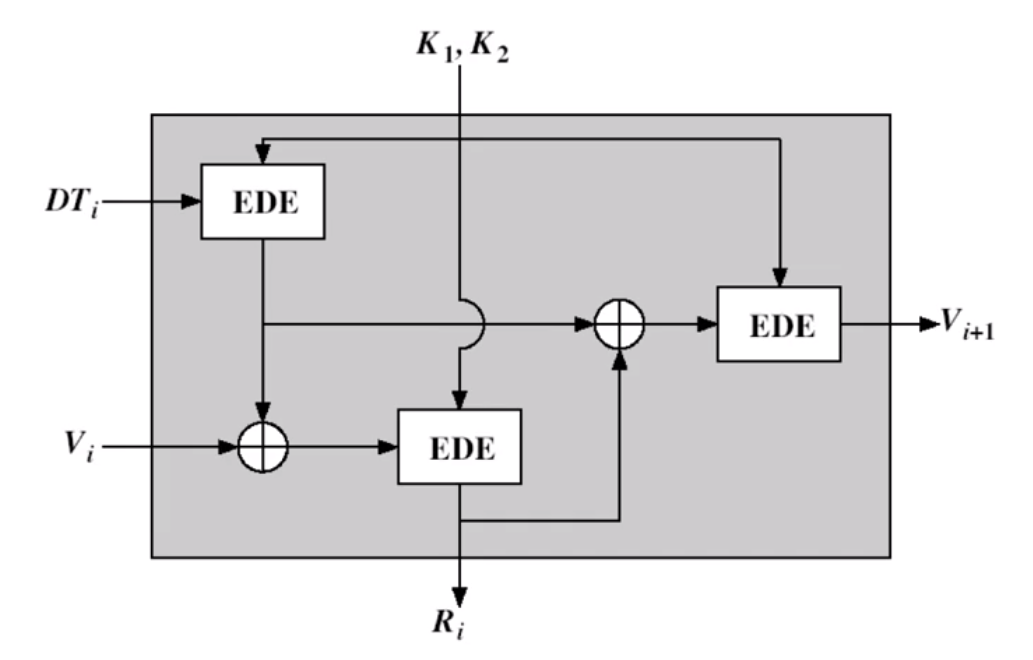
\includegraphics[width=0.9\linewidth]{immagini/img47}
	\centering
\end{figure}

La crittoanalisi è molto complicata.

BBS balza

\subsection*{Crittosistemi a chiave pubblica}
\addcontentsline{toc}{subsection}{Crittosistemi a chiave pubblica}
Il problema dei sistemi simmetrici è che Alice e Bob devono conoscere la stessa chiave $k$. Serve quindi un canale privato (quindi sicuro) per comunicarsi la chiave, e questo non è sempre possibile. La crittografia a chiave pubblica risolve questo sistema: non c'è bisogno di un canale privato.

L'idea è che ogni utente crea attraverso un algoritmo una coppia di chiavi, la chiave di cifratura è pubblica, la chiave di decifratura rimane segreta. Quindi tutti possono cifrare un messaggio, ma solo io che conosco la chiave segreta posso decifrarlo.


Vediamo due soluzioni:\\
Bob ha due algoritmi:
\begin{itemize}
	\item $E_B$: cifratura
	\item $D_B$: decifratura
\end{itemize}
tali per cui $D_B$ decifra i messaggi cifrati con $E_B$.
Se Alice vuole mandare un messaggio $m$ a Bob, gli chiede $E_B$ e calcola $E_B(m)$. Successivamente lo invia e Bob calcola $D_B(E_B(m)) = m$.\\
Se Eve intercetta $E_B(m)$ dovrebbe risolvere un problema che abbiamo assunto essere infattibile.
Il problema è che in una grande rete di utenti Alice deve chiedere a tutti i loro algoritmi di cifratura.

Seconda soluzione:\\
Alice e Bob scelgono un algoritmo di cifratura e un algorimo di decifratura.
I due algoritmi di decifratura/cifratura commutano, quindi possono essere scambiati.
\begin{enumerate}
	\item Alice calcola $E_A(m)$ e lo manda a Bob
	\item Bob lo cifra con $E_B$ e lo rimanda ad Alice
	\item Alice riceve $E_B(E_A(m))$, applica $D_A$ e manda a Bob
	\item Bob applica $D_B$ e ottiene $D_B(D_A(E_B(E_A(m)))) = D_A(E_A(m)) = m$
\end{enumerate}
Lo svantaggio è che i messaggi vanno avanti e indietro due volte, però ognuno tiene il suo algoritmo di cifratura e può cambiarlo quando vuole.

Il problema è che il canale non è autenticato: quando Alice riceve la chiave pubblica di Bob, come fa ad essere sicura che non abbia ricevuto invece quelle di Eve?

Definizione formale di one-way function:
$f$ può essere computata in tempo polinomiale da una MDT, ed esistono due polinomi $p(\dot)$ e $q(\dot)$ tali per cui $p(|x|) \leq |f(x)| \leq q(|x|)$ (quindi l'output di $f$ non dev'essere troppo corto).

Per ogni algoritmo $A$ dell'attaccante che può essere eseguito in tempo polinomiale su una macchina probabilitstica TM e per ogni polinomio $p(\dot)$ esiste un numero $n_{A,p}$ tale per cui:
\begin{equation*}
\forall n \geq n_{A,p} \; \; Prob[x \leftarrow \{0,1\}^n; x'\leftarrow A(f(x)):f(x)=f(x')] \leq \frac1{p(n)}
\end{equation*}

Il problema è che se $P=NP$ allora le funzioni one-way non esistono! Se però si dimostra che una one-way function esiste allora $P \neq NP$